\scanpage{121}
\mspage{III-42}
En outre, on sait que $H^i(X,\underline F)=0$ sauf pour un nombre fini de valeurs de $i$ (\uline{loc.cit.}) ; le nombre entier
\[
(15)\qquad\chi_A(\underline F)=\sum_{i=0}^{\infty}(-1)^i\operatorname{Long}(H^i(X,\underline F))
\]
est donc défini pour tout $\underline O_X$-module cohérent $\underline F$ ; on l'appelle la \uline{caractéristique d'Euler-Poincaré de $\underline F$} (\uline{par rapport à l'anneau A}).
\margin{si $A$ est local}
\figure{\begin{tikzpicture}[x=.6cm,y=.6cm]\draw(0,0)--(.1,1.5);\draw(.1,1.5)circle(.08);\draw(5,0)--(5.5,1.4);\draw(5.5,1.4)circle(.08);\end{tikzpicture}}
Pour $\underline F=\underline O_X$, on dit que $\chi_A(\underline O_X)$ est le \uline{genre} \deleted{\illegible{1}} \uline{arithmétique} de $X$.

\uline{Proposition 13 .- Soit} $0\to\underline{F'}\to\underline F\to\underline{F''}\to0$ \uline{une suite exacte de $\underline O_X$-modules cohérents. On a alors}
\[
(16)\qquad\chi_A(\underline F)=\chi_A(\underline{F'})+\chi_A(\underline{F''}).
\]
On a en effet, par la suite exacte de cohomologie, une suite \unsure{exacte}
\[
\begin{gathered}
0\to H^0(X,\underline{F'})\to H^0(X,\underline F)\to H^0(X,\underline{F''})\to H^1(X,\underline{F'})\to\cdots\\
\to H^r(X,\underline{F'})\to H^r(X,\underline F)\to H^r(X,\underline{F''})\to0
\end{gathered}
\]
\deleted{\illegible{1}} les modules de cohomologie d'indice $>r$ étant nuls pour $\underline F$, $\underline{F'}$ et $\underline{F''}$. Or on sait que dans une suite exacte de modules de longueur finie, ayant des 0 aux deux extrémités, la somme alternée des longueurs est nulle ; appliquant ce résultat, on trouve immédiatement (16).

\uline{Théorème 2 .-} \inserted{\uline{Soit $\underline F$ un $\underline O_X$-module cohérent}.}
(i) \deleted{\illegible{3}} \uline{La fonction} $n\to\chi_A(\underline F(n))$ \uline{est \inserted{égale à} un polynôme \inserted{en $n$}.}

(ii) \uline{Pour n assez grand, on a} $\chi_A(\underline F(n))=\operatorname{Long}\Gamma(X,\underline F(n))$ ; \uline{si} $\underline F=\widetilde M$, \deleted{\illegible{2}} (\uline{où M est un S-module gradué de type fini}), \uline{on a} $\chi_A(\underline F(n))=\operatorname{Long}(M_n)$ \uline{pour n assez grand}.

(iii) \uline{Le terme de plus haut degré de} $\chi_A(\underline F(n))$ \uline{a un coefficient} $\geq0$.
\margin{$>$}

(iv) \uline{Le degré de} $\chi_A(\underline F(n))$ \uline{est égale à la dimension du support de $\underline F$}.

Soient \deleted{$\unsure{z}$} $\xi_1,\ldots,\xi_m$ les points de $Z=\operatorname{Spec}(A)$ ; on sait que \deleted{$\unsure{Z}$} $Z$ est somme des schémas $Z_i=\operatorname{Spec}(A_i)$, \deleted{\unsure{et}} où \deleted{\unsure{les}} les $A_i$ sont les composants locaux de $A$, et l'espace de base de $Z_i$ est $\{\xi_i\}$ (I,4,1,prop.4) ; si $f:X\to Z$ est le morphisme structural, $X$ est alors somme des présché-
\margin{Joube}
\figure{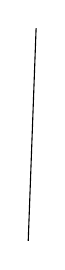
\begin{tikzpicture}\draw(0,0)--(.1,2.7);\end{tikzpicture}}
\mspage{120}

